\chapter{Experiments}\label{chap:experiments}
Declaration files were generated for existing modules repository. The DefinitelyTyped repository was used as a benchmark. Each one of the generated files was compared against the corresponding declaration file already uploaded to the repository.

\figref{fig:experiments-overall-funnel} shows that a declaration file was generated for 244 modules out of 6029. The following sections explain each stage of the process. Examples of generated declaration files for existing modules are presented in \secref{sec:experiments-declaration-files-generation}.

\definecolor{myellow}{RGB}{228,212,0}
\definecolor{mgreen}{RGB}{5,104,57}

\newcommand\funnel[3]{%
\pgfmathsetmacro\mwid{(0.3+\val*0.06)}
\pgfmathsetmacro\mradius{(\val*0.01 + 1)}
\pgfmathsetmacro\mheight{(\val*0.003 + 0.4)}
\pgfmathsetmacro\marc{\mwid-.4}
    \begin{scope}[%
        shift={(0,#1)}, 
        line width=.05pt, 
        %x=5mm, 
        %scale=1.\xi,
        yshift=\xi*4
        ]
    \draw[black,bottom color=#2, top color=#2] (-\mwid,0) -- (-\mwid+.4,-\mheight) arc (190:350:\marc cm and \mradius mm) -- (\mwid,0);
    \draw[black,fill=#3] (0,0) ellipse (\mwid cm and \mradius mm);
    \path (-\mwid,0) -- (-\mwid+.4,-\mheight) coordinate[midway] (a\xi);
    \end{scope}
}

\begin{figure}[tp]
	\hspace*{-0.28\textwidth}
	\centering
	\begin{tikzpicture}
		\foreach \val
				[%
				count=\xi starting from 0, 
				evaluate=\xi as \shadecolor using int(25*\xi),
				evaluate=\xi as \coord using int(\xi-12)
				]
			in {
				4.05,
				7.33,
				24.02,
				37.49,
				71.19,
				82.50,
				100.00
			}{
				\funnel{\coord}{mgreen!\shadecolor !myellow}{mgreen!\shadecolor !myellow}
			}   

		\node[left=0.02\textwidth of a0] {Generated Declaration Files};
		\node[right=0.07\textwidth of a0] {\textbf{244}};

		\node[left=0.02\textwidth of a1] {Run-time Information};
		\node[right=0.12\textwidth of a1] {\textbf{442}};

		\node[left=0.02\textwidth of a2] {Working Examples};
		\node[right=0.26\textwidth of a2] {\textbf{1448}};

		\node[left=0.02\textwidth of a3] {Code Examples};
		\node[right=0.38\textwidth of a3] {\textbf{2260}};

		\node[left=0.02\textwidth of a4] {README file};
		\node[right=0.70\textwidth of a4] {\textbf{4292}};

		\node[left=0.02\textwidth of a5] {Github Repository};
		\node[right=0.80\textwidth of a5] {\textbf{4974}};

		\node[align=right,left=0.02\textwidth of a6, text width=0.25\textwidth] {Definitely Typed Modules};
		\node[right=0.97\textwidth of a6] {\textbf{6029}};

	\end{tikzpicture}
	\caption[Number of analyzed modules for each stage of the experiment]{\textbf{Number of analyzed modules for each stage of the experiment} - A TypeScript Declaration File was generated for only 244 modules, out of 6029 modules in the DefinitelyTyped Repository. It was possible to gather valid run-time information for only 25\% of the modules for which a Code Example was extracted.}
	\label{fig:experiments-overall-funnel}
\end{figure}

An analysis on the usage of JavaScript operators can be seen in \secref{sec:experiments-js-operators-usage}.

\section{Definitely Typed Benchmark}

\draft{Chequear modulo 'acl' por ejempo que tiene errores y esta exportado como module pero deberia ser exportado como module-class. Habia otro modulo pero no lo recuerdo.}


\subsection{Code Examples Extraction}
Extracting the code examples from the repositories of the JavaScript libraries proved to be a pragmatic way of capturing the types. However, code examples for only 2260 out of 6029 modules could be retrieved.

\subsubsection{Repositories URL}
The url of the repositories could be retrieved for only 4974 modules. More than 1000 modules do not have the repository entry in their corresponding \mintinline{text}{package.json} files. Therefore, the \mintinline{text}{npm view <module> repository.url} command returns an empty value. This is even happening for important modules like \mintinline{text}{ace}.

\subsubsection{Readme Files}
700 modules simply do not have a readme file in their repositories. The implementation does contemplate, however, different naming conventions like \mintinline{text}{readme.md} or \mintinline{text}{README.md}.

\subsubsection{Code Examples Extraction}
The 50\% loss is mainly explained because developers did not tag their code around the \mintinline{text}{javascript} tag in their markdown readme files. As explained in \secref{sec:conclusions-future-work}, the process of extracting code examples from a repository can be greatly improved. Counting with code examples for 2200 modules was considered to be enough for this work.

\subsubsection{Code Examples Execution}
Only 1448 modules had working code examples. The 2260 extracted code examples were executed by installing the required packages and running the code as a \mintinline{text}{node} application. 812 modules did not run correctly and were discarded from the analysis. Some failing examples were analyzed and there were mainly two reasons for the failure: 1) The code example had been properly extracted but the code itself was not working properly and 2) the extracted code example was not correct.
Improving the retrieval the code examples for a specific module will definitely have a positive impact in this number.

\subsection{Run-time Information Gathering} \label{sec:experiments-run-time-information-gathering}
Run-time information could only be extracted for 442 modules out of 1448 modules with working code examples. As explained in \secref{sec:run-time-wrapper-objects}, the behavior of the code under analysis was explicitly modified by wrapping the arguments around Wrapper Objects. This definitely had an influence on the executed code of some modules by causing new run-time errors. Furthermore, Jalangi's own limitation in the instrumentation process caused some of the modules to be unable to be instrumented.

A plain Jalangi instrumentation, i.e. without user defined analysis modules, was not applied to the 1448 working code examples. Therefore, it was not possible to determine which modules are failing only because of Jalangi's own limitations.

\subsection{Declaration Files Generation} \label{sec:experiments-declaration-files-generation}
Finally, a declaration file was generated for 244 modules. Despite the correct gathering of run-time information, some of the 442 modules mentioned in \secref{sec:experiments-run-time-information-gathering} did not contain valid run-time information for the generation of the declaration file. The main reason for this behavior is that the extracted code examples did not execute the modules in a way that which gathers valid run-time information.

\subsection{Evaluation}
As shown in \figref{fig:experiments-typescript-templates-distribution-definitely-typed}, 72\% of the modules uploaded to DefinitelyTyped are written using the \mintinline{text}{modules} template. On the other hand, 20\% of them are written using the \mintinline{text}{module-function}. The complexity of evaluating declaration files written with the \mintinline{text}{module-function} is considerably lower than for the other templates. Templates \mintinline{text}{module-class} and \mintinline{text}{module} were not evaluated. 20\% was considered enough as a starting point.

\begin{figure}[tp]
	\centering
	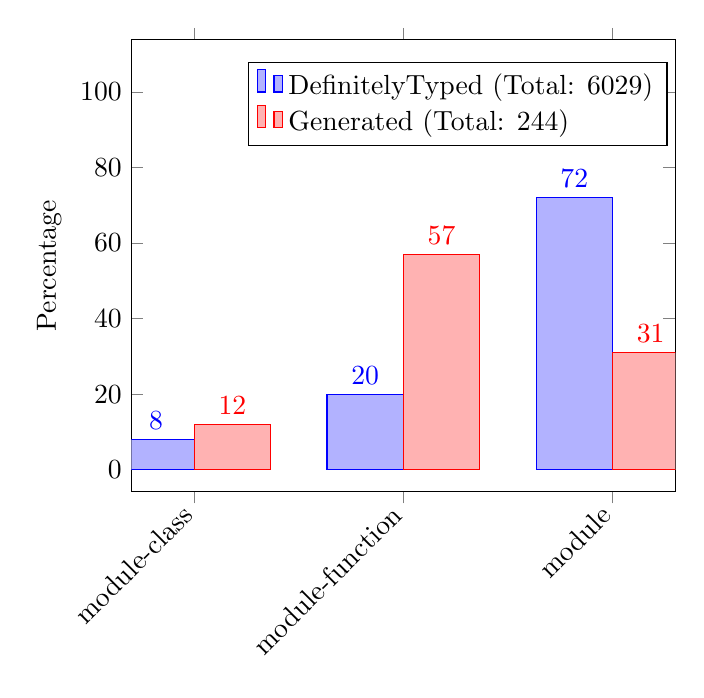
\begin{tikzpicture}
		\begin{axis}[
			ybar,
			width=0.7\textwidth,
			ybar=0pt,
			ymax=100,
			enlargelimits=0.15,
			bar width=0.08\textwidth,
			legend columns=1,
			legend cell align={left},
			legend style={at={(0.6,0.95)}, anchor=north},
			symbolic x coords={module-class,module-function,module},
			xtick=data,
			ylabel=Percentage,
			nodes near coords, 
			nodes near coords align={vertical},
			x tick label style={rotate=45,anchor=east},
		]
		\addplot coordinates {
			(module-class, 8)
			(module-function, 20)
			(module, 72)
		};

		\addplot coordinates {
			(module-class, 12)
			(module-function, 57)
			(module, 31)
		};
		\legend{DefinitelyTyped (Total: 6029), Generated (Total: 244)}
		\end{axis}
	\end{tikzpicture}

	\caption[TypeScript templates distribution | Generated \& DefinitelyTyped]{\textbf{TypeScript templates distribution | Generated \& DefinitelyTyped} - Out of a total of 6029, 72\% of the modules uploaded to the DefinitelyTyped repository use the \mintinline{text}{module} template and only 20\% use the \mintinline{text}{module-function} one. However, 57\% of the 244 generated declaration files use the \mintinline{text}{module-function} template.
	}

	\label{fig:experiments-typescript-templates-distribution-definitely-typed}
\end{figure}

\subsection{Results}

\begin{figure}[tp]
	\centering
	\begin{lrbox}{\mintedbox}
		\begin{minipage}{0.49\textwidth}
			\tscode{code/experiments/results/module-function/abs/generated.d.ts}
		\end{minipage}
	\end{lrbox}
	\subfloat[abs/index.d.ts - Generated]{\usebox{\mintedbox}}
	\hfill
	\begin{lrbox}{\mintedbox}
		\begin{minipage}{0.49\textwidth}
			\tscode{code/experiments/results/module-function/abs/definitely-typed.d.ts}
		\end{minipage}
	\end{lrbox}
	\subfloat[abs/index.d.ts - DefinitelyTyped]{\usebox{\mintedbox}}

	\begin{lrbox}{\mintedbox}
		\begin{minipage}{0.49\textwidth}
			\tscode{code/experiments/results/module-function/dirname-regex/generated.d.ts}
		\end{minipage}
	\end{lrbox}
	\subfloat[dirname-regex/index.d.ts - Generated]{\usebox{\mintedbox}}
	\hfill
	\begin{lrbox}{\mintedbox}
		\begin{minipage}{0.49\textwidth}
			\tscode{code/experiments/results/module-function/dirname-regex/definitely-typed.d.ts}
		\end{minipage}
	\end{lrbox}
	\subfloat[dirname-regex/index.d.ts - DefinitelyTyped]{\usebox{\mintedbox}}

	\begin{lrbox}{\mintedbox}
		\begin{minipage}{0.49\textwidth}
			\tscode{code/experiments/results/module-function/escape-html/generated.d.ts}
		\end{minipage}
	\end{lrbox}
	\subfloat[escape-html/index.d.ts - Generated]{\usebox{\mintedbox}}
	\hfill
	\begin{lrbox}{\mintedbox}
		\begin{minipage}{0.49\textwidth}
			\tscode{code/experiments/results/module-function/escape-html/definitely-typed.d.ts}
		\end{minipage}
	\end{lrbox}
	\subfloat[escape-html/index.d.ts - DefinitelyTyped]{\usebox{\mintedbox}}

	\caption[Module-function results]{\textbf{Module-function results} - Results are shown for modules \mintinline{text}{abs}, \mintinline{text}{dirname-regex}, \mintinline{text}{escape-html}. On the left side the generated declaration file with \mintinline{text}{dts-generate}. On the right side the corresponding file in the DefinitelyTyped repository. Functions are correctly detected and input types are accurately inferred. Both files are parsed for comparison, as explained in \secref{sec:approach-parsing}. Therefore, subtle differences in the syntax between both files are not important.}
	\label{fig:experiments-results-module-function}
\end{figure}

\begin{figure}[tp]
	\centering
	\begin{lrbox}{\mintedbox}
		\begin{minipage}{0.8\textwidth}
			\tscode{code/experiments/results/module-class/flake-idgen/generated.d.ts}
		\end{minipage}
	\end{lrbox}
	\subfloat[flake-idgen/index.d.ts - Generated]{\usebox{\mintedbox}}

	\begin{lrbox}{\mintedbox}
		\begin{minipage}{0.8\textwidth}
			\tscode{code/experiments/results/module-class/flake-idgen/definitely-typed.d.ts}
		\end{minipage}
	\end{lrbox}
	\subfloat[flake-idgen/index.d.ts - DefinitelyTyped]{\usebox{\mintedbox}}

	\caption[Module-class results | flake-idgen]{\textbf{Module-class results | flake-idgen} - Parameters of interface \mintinline{text}{ConstructorOptions} are correctly detected. Name of interface differs since it is automatically generated based on the name of the argument variable. Optional properties were not implemented, hence the \mintinline{text}{undefined} type for some properties. Analogously, callback \mintinline{text}{cb} is inferred as \mintinline{text}{undefined}.}
	\label{fig:experiments-results-module-class-flake-idgen}
\end{figure}

\begin{figure}[tp]
	\centering
	\begin{lrbox}{\mintedbox}
		\begin{minipage}{0.8\textwidth}
			\tscode{code/experiments/results/module-class/route-parser/generated.d.ts}
		\end{minipage}
	\end{lrbox}
	\subfloat[route-parser/index.d.ts - Generated]{\usebox{\mintedbox}}

	\begin{lrbox}{\mintedbox}
		\begin{minipage}{0.8\textwidth}
			\tscode{code/experiments/results/module-class/route-parser/definitely-typed.d.ts}
		\end{minipage}
	\end{lrbox}
	\subfloat[route-parser/index.d.ts - DefinitelyTyped]{\usebox{\mintedbox}}

	\caption[Module-class results | route-parser]{\textbf{Module-class results | route-parser} - Constructor and methods are correctly identified. Specific signature of dictionary \mintinline{text}{params} is not detected. Instead, a generic \mintinline{text}{object} is inferred.}
	\label{fig:experiments-results-module-class-route-parser}
\end{figure}

\begin{figure}[tp]
	\centering
	\begin{lrbox}{\mintedbox}
		\begin{minipage}{0.8\textwidth}
			\tscode{code/experiments/results/module-class/timer-machine/generated.d.ts}
		\end{minipage}
	\end{lrbox}
	\subfloat[timer-machine/index.d.ts - Generated]{\usebox{\mintedbox}}

	\begin{lrbox}{\mintedbox}
		\begin{minipage}{0.8\textwidth}
			\tscode{code/experiments/results/module-class/timer-machine/definitely-typed.d.ts}
		\end{minipage}
	\end{lrbox}
	\subfloat[timer-machine/index.d.ts - DefinitelyTyped]{\usebox{\mintedbox}}

	\caption[Module-class results | timer-machine]{\textbf{Module-class results | timer-machine} - Parameter \mintinline{text}{started} is inferred as \mintinline{text}{undefined} instead of marking it as optional. Methods that were not executed do not appear in the generated declaration file.}
	\label{fig:experiments-results-module-class-timer-machine}
\end{figure}

\begin{figure}[tp]
	\centering
	\begin{lrbox}{\mintedbox}
		\begin{minipage}{0.8\textwidth}
			\tscode{code/experiments/results/module/is-uuid/generated.d.ts}
		\end{minipage}
	\end{lrbox}
	\subfloat[is-uuid/index.d.ts - Generated]{\usebox{\mintedbox}}

	\begin{lrbox}{\mintedbox}
		\begin{minipage}{0.8\textwidth}
			\tscode{code/experiments/results/module/is-uuid/definitely-typed.d.ts}
		\end{minipage}
	\end{lrbox}
	\subfloat[is-uuid/index.d.ts - DefinitelyTyped]{\usebox{\mintedbox}}

	\caption[Module results | is-uuid]{\textbf{Module results | is-uuid} - Methods that were not executed are not included in the declaration file.}
	\label{fig:experiments-results-module-is-uuid}
\end{figure}

\begin{figure}[tp]
	\centering
	\begin{lrbox}{\mintedbox}
		\begin{minipage}{0.49\textwidth}
			\tscode{code/experiments/results/module/datadog-metrics/generated.d.ts}
		\end{minipage}
	\end{lrbox}
	\subfloat[datadog-metrics/index.d.ts - Generated]{\usebox{\mintedbox}}
	\hfill
	\begin{lrbox}{\mintedbox}
		\begin{minipage}{0.49\textwidth}
			\tscode{code/experiments/results/module/datadog-metrics/definitely-typed.ts}
		\end{minipage}
	\end{lrbox}
	\subfloat[datadog-metrics/index.d.ts - DefinitelyTyped]{\usebox{\mintedbox}}

	\begin{lrbox}{\mintedbox}
		\begin{minipage}{0.95\textwidth}
			\tscode{code/experiments/results/module/datadog-metrics/logger-datadog-metrics.js}
		\end{minipage}
	\end{lrbox}
	\subfloat[datadog-metrics/logger.js]{\usebox{\mintedbox} \label{fig:subfloat-datadog-logger} }

	\caption[Missing properties | datadog-metrics]{\textbf{Missing properties | datadog-metrics} - Properties \mintinline{text}{aggregator} and \mintinline{text}{reporter} are not in the DefinitelyTyped version, but they appear in the generated declaration file. However, they are indeed used by the library, as exposed in lines 2 and 3 of the library's source code shown in \protect\subref{fig:subfloat-datadog-logger}.}
	\label{fig:experiments-results-module-datadog-metrics}
\end{figure}

\section{JS Operators Usage} \label{sec:experiments-js-operators-usage}
\todo{Agregar que es una matriz simetrica. Que era para hacer un analisis mas global. Para algunos operators se puede inferir que el orden de los tipos sí afecta. Por ejemplo para instance of donde obviamente importa el orden. Pero para == por ejemplo generalmente se pone a == null y no null == a}.
\input{figures/experiments/operators/relational-operators/relationalOperators.tex}
\begin{figure}[tp]
	\centering

	\begin{tikzpicture}
		\begin{axis}[
			view={0}{90},
			title=Operator ${+}$,
			width=0.45\textwidth,
			colormap/hot,
			xticklabels={number,string,undefined,object,null,boolean,function,array},
			xtick={0,...,7},
			yticklabels={number,string,undefined,object,null,boolean,function,array},
			ytick={7,...,0},
			x tick label style={rotate=90,anchor=east}]
		]
		\addplot3[surf, shader=interp, left] file {figures/experiments/operators/additive-operators/operator_+.dat};
		\end{axis}
	\end{tikzpicture}
	%
	\begin{tikzpicture}
		\begin{axis}[
			view={0}{90},
			width=0.45\textwidth,
			title=Operator ${-}$,
			colormap/hot,
			xticklabels={number,string,undefined,object,null,boolean,function,array},
			xtick={0,...,7},
			yticklabels={number,string,undefined,object,null,boolean,function,array},
			ytick={7,...,0},
			x tick label style={rotate=90,anchor=east}]
		\addplot3[surf, shader=interp, left] file {figures/experiments/operators/additive-operators/operator_-.dat};
		\end{axis}
	\end{tikzpicture}

	\centering
	\hspace{0.1\textwidth}
	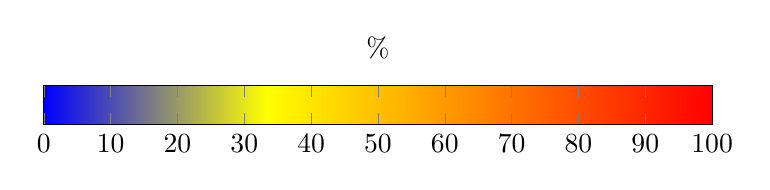
\begin{tikzpicture}
		\begin{axis}[
			hide axis,
			scale only axis,
			height=0pt,
			width=0pt,
			colormap/hot,
			colorbar horizontal,
			point meta min=0,
			point meta max=100,
			colorbar style={
				title=\%,
				width=0.7\textwidth,
				xtick={0, 10, 20, 30, 40, ..., 100}
			}]
			\addplot [draw=none] coordinates {(0,0)};
		\end{axis}
	\end{tikzpicture}
	\caption[Additive operators]{\textbf{Type distribution for additive operators} - Both operators are mainly used with the \textit{number-number} combination. Operator $+$ is also used for pure string concatenation. However, due to JS Type Coercion, $+$ is also used for \textit{string} and \textit{number} concatenation}
	\label{fig:experiments-additive-operators}
\end{figure}
\begin{figure}[tp]
	\centering

	\begin{tikzpicture}
		\begin{axis}[
			view={0}{90},
			title=Operator ${*}$,
			width=0.45\textwidth,
			colormap/hot,
			xticklabels={number,string,undefined,object,null,boolean,function,array},
			xtick={0,...,7},
			yticklabels={number,string,undefined,object,null,boolean,function,array},
			ytick={7,...,0},
			x tick label style={rotate=90,anchor=east}]
		]
		\addplot3[surf, shader=interp, left] file {figures/experiments/operators/multiplicative-operators/operator_star.dat};
		\end{axis}
	\end{tikzpicture}
	%
	\begin{tikzpicture}
		\begin{axis}[
			view={0}{90},
			width=0.45\textwidth,
			title=Operator ${/}$,
			colormap/hot,
			xticklabels={number,string,undefined,object,null,boolean,function,array},
			xtick={0,...,7},
			yticklabels={number,string,undefined,object,null,boolean,function,array},
			ytick={7,...,0},
			x tick label style={rotate=90,anchor=east}]
		\addplot3[surf, shader=interp, left] file {figures/experiments/operators/multiplicative-operators/operator_division.dat};
		\end{axis}
	\end{tikzpicture}

	\centering
	\begin{tikzpicture}
		\begin{axis}[
			view={0}{90},
			width=0.45\textwidth,
			title=Operator ${\%}$,
			colormap/hot,
			xticklabels={number,string,undefined,object,null,boolean,function,array},
			xtick={0,...,7},
			yticklabels={number,string,undefined,object,null,boolean,function,array},
			ytick={7,...,0},
			x tick label style={rotate=90,anchor=east}]
		\addplot3[surf, shader=interp, left] file {figures/experiments/operators/multiplicative-operators/operator_percentage.dat};
		\end{axis}
	\end{tikzpicture}
	
	\centering
	\hspace{0.1\textwidth}
	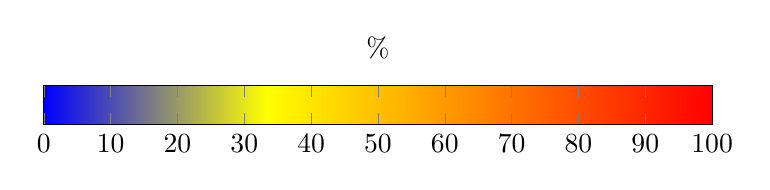
\begin{tikzpicture}
		\begin{axis}[
			hide axis,
			scale only axis,
			height=0pt,
			width=0pt,
			colormap/hot,
			colorbar horizontal,
			point meta min=0,
			point meta max=100,
			colorbar style={
				title=\%,
				width=0.7\textwidth,
				xtick={0, 10, 20, 30, 40, ..., 100}
			}]
			\addplot [draw=none] coordinates {(0,0)};
		\end{axis}
	\end{tikzpicture}
	\caption[Relational operators]{\textbf{Type distribution for multiplicative operators} - All multiplicative operators are mainly used with the \textit{number-number} combination}
\end{figure}
\begin{figure}[tp]
	\centering

	\begin{tikzpicture}
		\begin{axis}[
			view={0}{90},
			title=Operator ${==}$,
			width=0.45\textwidth,
			colormap/hot,
			xticklabels={number,string,undefined,object,null,boolean,function,array},
			xtick={0,...,7},
			yticklabels={number,string,undefined,object,null,boolean,function,array},
			ytick={7,...,0},
			x tick label style={rotate=90,anchor=east}]
		]
		\addplot3[surf, shader=interp, left] file {figures/experiments/operators/equality-operators/operator_==.dat};
		\end{axis}
	\end{tikzpicture}
	%
	\begin{tikzpicture}
		\begin{axis}[
			view={0}{90},
			width=0.45\textwidth,
			title=Operator ${!=}$,
			colormap/hot,
			xticklabels={number,string,undefined,object,null,boolean,function,array},
			xtick={0,...,7},
			yticklabels={number,string,undefined,object,null,boolean,function,array},
			ytick={7,...,0},
			x tick label style={rotate=90,anchor=east}]
		\addplot3[surf, shader=interp, left] file {figures/experiments/operators/equality-operators/operator_!=.dat};
		\end{axis}
	\end{tikzpicture}

	\centering
	\begin{tikzpicture}
		\begin{axis}[
			view={0}{90},
			width=0.45\textwidth,
			title=Operator ${===}$,
			colormap/hot,
			xticklabels={number,string,undefined,object,null,boolean,function,array},
			xtick={0,...,7},
			yticklabels={number,string,undefined,object,null,boolean,function,array},
			ytick={7,...,0},
			x tick label style={rotate=90,anchor=east}]
		\addplot3[surf, shader=interp, left] file {figures/experiments/operators/equality-operators/operator_===.dat};
		\end{axis}
	\end{tikzpicture}
	%
	\begin{tikzpicture}
		\begin{axis}[
			view={0}{90},
			width=0.45\textwidth,
			title=Operator ${!==}$,
			colormap/hot,
			xticklabels={number,string,undefined,object,null,boolean,function,array},
			xtick={0,...,7},
			yticklabels={number,string,undefined,object,null,boolean,function,array},
			ytick={7,...,0},
			x tick label style={rotate=90,anchor=east}]
		\addplot3[surf, shader=interp, left] file {figures/experiments/operators/equality-operators/operator_!==.dat};
		\end{axis}
	\end{tikzpicture}

	\centering
	\hspace{0.1\textwidth}
	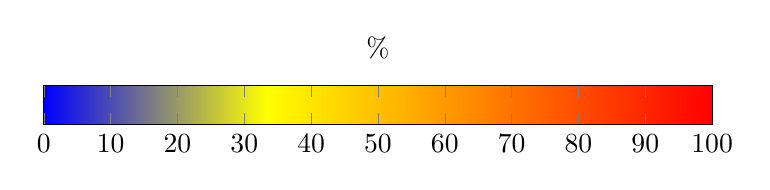
\begin{tikzpicture}
		\begin{axis}[
			hide axis,
			scale only axis,
			height=0pt,
			width=0pt,
			colormap/hot,
			colorbar horizontal,
			point meta min=0,
			point meta max=100,
			colorbar style={
				title=\%,
				width=0.7\textwidth,
				xtick={0, 10, 20, 30, 40, ..., 100}
			}]
			\addplot [draw=none] coordinates {(0,0)};
		\end{axis}
	\end{tikzpicture}
	\caption[Relational operators]{
		\textbf{Type distribution for equality operators} - Operator ${==}$ is mainly used for number comparison. String comparison is performed by using ${===}$ and ${!==}$ operators. Comparison against \textit{null} is performed by using both ${!=}$ and ${!==}$ operators
	}
	\label{fig:experiments-equality-operators}
\end{figure}
\begin{figure}[tp]
	\centering
	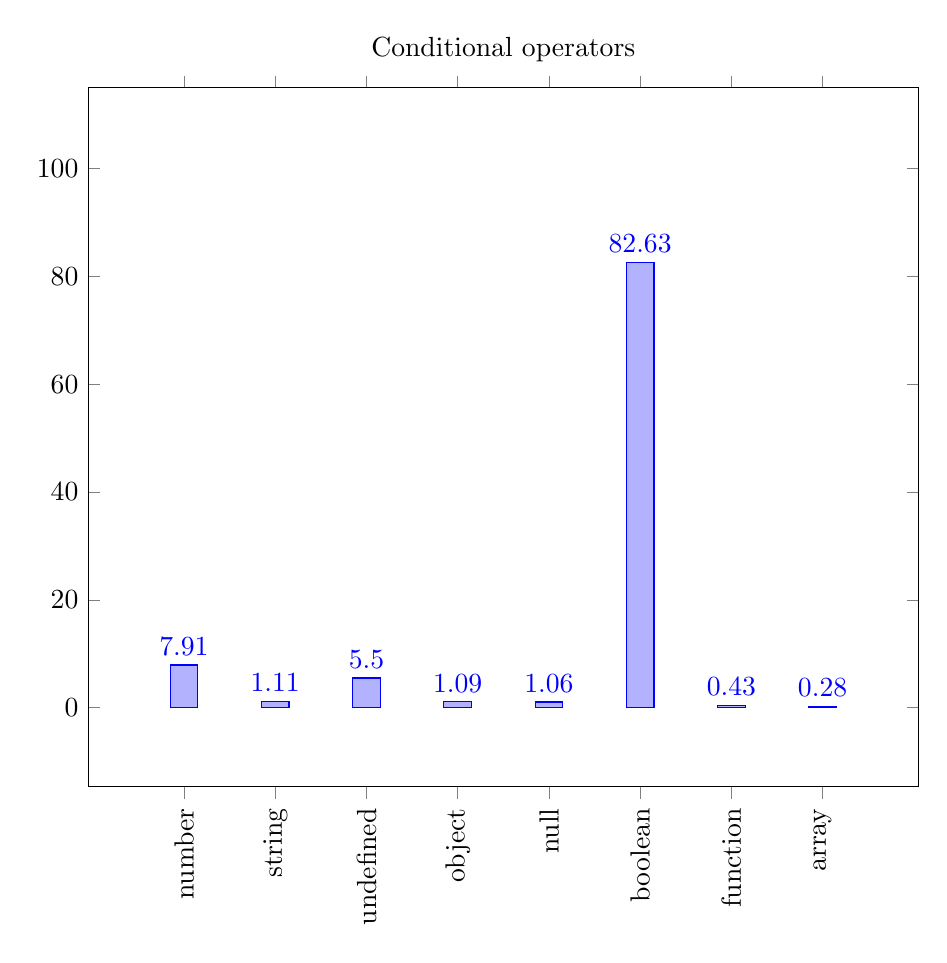
\begin{tikzpicture}
		\begin{axis}[
			ybar,
			title=Conditional operators,
			width=1\textwidth,
			ybar=0pt,
			ymax=100,
			enlargelimits=0.15,
			legend style={at={(0.5,-0.2)}, anchor=north,legend columns=-1},
			symbolic x coords={number,string,undefined,object,null,boolean,function,array},
			xtick=data,
			nodes near coords, 
			nodes near coords align={vertical},
			x tick label style={rotate=90,anchor=east},
		]
		\addplot coordinates {
			(number, 7.91)
			(string, 1.11)
			(undefined, 5.50)
			(object, 1.09)
			(null, 1.06)
			(boolean, 82.63)
			(function, 0.43)
			(array, 0.28)
		};
		\end{axis}
	\end{tikzpicture}
	\caption[Conditional operators]{\textbf{Type distribution for conditional operators} - It includes all operators that trigger a condition check before branching: ${if-then-else}$, ${switch-case}$, ${while}$, ${for}$, ${||}$, ${\&\&}$, ${ ? : }$.
	}
\end{figure}